% The CJAM .tex template. Adapted from the JASA template. The .tex file for JASA can be found at:
% https://www.overleaf.com/latex/templates/journal-of-the-american-statistical-association-jasa-template/tmwhhgvxwwvc


\documentclass[12pt]{article}
\usepackage{amsmath}
\usepackage{graphicx,psfrag,epsf}
\usepackage{enumerate}
\usepackage{float}
\usepackage{url} % not crucial - just used below for the URL
\usepackage{lipsum}  %not crucial - just used to generate dummy text in section 3


%DON'T CHANGE MARGIN
\usepackage[margin = 1in]{geometry}

\begin{document}


\def\spacingset#1{\renewcommand{\baselinestretch}%
{#1}\small\normalsize} \spacingset{1}


%%%%%%%%%%%%%%%%%%%%%%%%%%%%%%%%%%%%%%%%%%%%%%%%%%%%%%%%%%%%%%%%%%%%%%%%%%%%%%

%%Define authors



  \title{\bf NCAA Basketball Team Rankings}
  \author{Scott Baker\thanks{
    The authors gratefully acknowledge Dr. Danielle Lyles.}\hspace{.2cm}\\
    Department of Applied Math, University of Colorado Boulder\\
    and \\
    Robert Hakulin \\
    Department of Aerospace, University of Colorado Boulder\\
    and \\
    Stian Howard \\
    Department of Computer Science, University of Colorado Boulder\\}
  \maketitle


\begin{abstract}
Every year, the NCAA selects 68 Division-I Men's basketball teams to compete in the final tournament. In this paper, the Colley Method is examined as a way of selecting teams that should progress to the tournament. The results from solving the Colley System are compared to the rankings provided by the NCAA tournament selection committee. Additionally, the results are also compared to another popular rating method---the ELO system. After sorting and processing over 11,000 games worth of data with a VBA Macro and computing the rankings by importing the data into MATLAB, it was found that the Colley method produced the same top 6 teams (in a slightly different order) as the NCAA committee. Furthermore,  these top 6 teams matched 5 of the top 6 teams put forward by the ELO system. Despite all systems having similar top teams, the ELO ratings deviate from the NCAA rankings more than the Colley ratings. This shows that streaks create weakness in the ELO system. Additionally, it is found that the Colley Method is a reliable, computationally-inexpensive way to rank teams similarly to how they are ranked by the NCAA.
\end{abstract}

\newpage
\spacingset{1.45} % DON'T change the spacing!
\section{Introduction}
\label{sec:intro} %allows for referencing previous (and forthcoming) sections in text
Each year, March Madness entertains and excites millions of fans while 68 NCAA Division-I Men's basketball teams battle on the court for a shot at the NCAA Championship. This two-week spectacle of basketball displays some of the best action a person can catch. However, out of the 351 teams in Division-I, only 68 teams make it to the tournament. How does the tournament selection committee accurately choose these teams?

Currently$^4$, the selection committee ranks teams based on record, strength of schedule, significant wins/losses, and previous tournament history. Strength of schedule means taking into account which teams a certain team has played and what the ranking of the opponent team is. This also ties into significant wins/losses. For example, if the top ranked team in the nation with a record of $10-0$ loses to a team that has a record of $0-10$, the committee will put more weight on this loss.
Previous tournament history means that the rankings of a certain team in a certain region can be affected by the team's all-time record at a certain stadium--one of which they may play at during the tournament. Basing the selection solely on wins and losses can be difficult because one team only plays about 35 games per season. Therefore, a certain team is unable to play all other teams. Being able to see trends and information about teams, conferences, and players have helped the ranking process become more accurate for the NCAA. However even though there are many factors that the selection committee uses in their rankings, this paper attempts to show that two different ranking systems, depending only on wins and losses, return similar results as the complicated NCAA selection.

One example of a method to rank teams is the Colley Method. This method involves a simple linear system:
\begin{equation}
C \vec{r} = \vec{b}
\end{equation}


In this linear system, $C$ is the Colley Matrix, $\vec{b}$ is a vector describing a certain team's win-loss relationship, and $\vec{r}$ a the ranking vector. Since the desired result is having rankings for teams, solving this system for $\vec{r}$ involves:

\begin{equation}
\vec{r} = C^{-1} \vec{b}
\label{eq:r}
\end{equation}


Then, the output $\vec{r}$ vector can be sorted to give final rankings of the teams observed. To look at the effectiveness of the Colley Method, this system was run in MATLAB on both small and large data sets with game results ranging from select schools to the entire Division-I bracket. Then, these sets were run with the ELO rating system and compared to the Colley Ratings. Finally, a complete, Division-I data set$^{2}$ that included results from all games played during the 2016-2017 season was run using the Colley Method and the ELO system. The results were then compared to the overall rankings given by the NCAA tournament selection committee. This provided insight into the effectiveness and accuracy of using the Colley Method to rank teams.














\section{The Colley Method}
\label{sec:meth}

As stated above, the general form of the Colley Method is solving the linear system $C$ $\vec{r}$ = $\vec{b}$ where $C$ is the Colley Matrix, $\vec{b}$ is a performance vector, and $\vec{r}$ is the desired ranking vector. To look deeper into this, first observe the general breakdown of $C$, the Colley Matrix:
\begin{center}
\[
C =
\begin{bmatrix}
2+t_1 & -n_{12} & -n_{13} & \hdots & -n_{1n}\\
-n_{21} & 2+t_2 & -n_{23} & \hdots & -n_{2n}\\
-n_{31} & -n_{32} & 2+t_3 & \hdots & -n_{3n}\\
\vdots & \vdots & \vdots & \ddots & \vdots\\
-n_{n1} & -n_{n2} & -n_{n3}& \hdots & 2+t_n
\end{bmatrix}
\]
\end{center}
~\\
This matrix is an $n$ $x$ $n$ matrix that corresponds with a system of $n$ teams. Entries along the diagonal are equal to $2 + t_i$ where $t_i$ is the total number of games team $i$ has played. All off-diagonal entries $c_{ij}$ are equal to $-n_{ij}$ where $n_{ij}$ is the number of games team $i$ has played team $j$. The result of this composition is that $C$ is a symmetric, positive definite matrix. This means this system is non-singular and therefore always has a solution. By always having a solution, the Colley Method will always output rankings for every team. Additionally for any row $i$,
the sum of the $n_{ij}$ entries equals $t_i$.
\begin{equation}
t_i = \Big\{\sum_{j=1}^{n} n_{ij} \mid i \neq j\Big\}
\end{equation}
This is a great way to check if the Colley Matrix has been set correctly. Furthermore since the matrix is symmetric, column $i$ behaves the same way. Next, the $\vec{b}$ vector is composed the following way:
\begin{center}
\[
\vec{b} =
\begin{bmatrix}
1 + \frac{1}{2}(w_1 - l_1)\\
\space\\
1 + \frac{1}{2}(w_2 - l_2)\\
\space\\
1 + \frac{1}{2}(w_3 - l_3)\\
\vdots\\
\vdots\\
1 + \frac{1}{2}(w_n - l_n)\\
\end{bmatrix}
\]
\end{center}

Each element, $b_i$, in $\vec{b}$ is made up by the expression $1 + \frac{1}{2}(w_i - l_i)$ where $w_i$ is the total number of wins and $l_i$ is the total number of losses for team $i$. The reason $\vec{b}$ is created like this is because it makes the average values over all the entries equal to 1.
\begin{equation}
\frac{1}{n}\sum_{i=1}^{n} b_{i} = 1
\end{equation}
By making $\vec{b}$ this way, the average value over the entries of the ranking vector is 0.5. The interpretation of this value is as follows. All possible $r_n$ values range from 0 to 1 in which the average value of the rank of a team as we observe more and more teams is a value of $0.5$. Furthermore, this statistic comes from the values of $r_n$ when there are no games played. In general, this comes from the following$^1$:

\begin{equation}
r = \frac{1 + n_w}{2 + n_{tot}}
\end{equation}

In which $n_w$ is the number of wins and $n_{tot}$ is the total number of games. At the beginning of the season, no teams have played and therefore all the rankings are $0.5$--also meaning that the average is $0.5$. The nature of this the $C$ matrix, in which a head-to-head matchup will affect both teams, creates the system so that the following is always true:

\begin{equation}
\frac{1}{n}\sum_{i=1}^{n} r_{i} = \frac{1}{2}
\end{equation}
Solving this system by left-multiplying by $C^{-1}$ outputs the values for $\vec{r}$. In order to find the top $n$ teams in the system, the values, $r_i$ in the ranking vector have to be sorted.

In general, the Colley Method is unbiased as it relies only on win-loss information for each team. It does not factor in unusual point differences. However, it only partially accounts for strength of schedule. Since the off-diagonal entries of the matrix can flag how many times a team plays another, it accounts for the overall comparison between those two teams based on the overall win-loss information for a team.
















\section{The ELO System}
\label{sec:elo}

In order to have another comparison for the Colley method and the teams chosen by the NCAA committee to play in the tournament, ELO rankings were determined for all the teams. The ELO system, which gained much respect starting in the 1930's, is similar to the Colley Method because it relies on win-loss information. The important difference between these methods is that the ELO system is based on game-by-game results and the Colley Method observes a whole set of games together. ELO is the choice system for most chess associations around the world and is often seen in sports-analytics systems such as FiveThirtyEight$^{5}$, ESPN for NCAA results and statistics, and NBA rankings from 1998 to 2013$^{6}$. Therefore, it should prove a reasonable standard for comparison.

The ELO system works by first assigning a player or team a standard number of points upon entry into the system--- common standards being 1000 and 1500, in which each team or player starts with the same value. From this point on, the system will calculate an expected win chance or result between two teams using the following equation:\\

\begin{equation}
E_A = \dfrac{1}{1+10^{\dfrac{R_B + R_A}{400}}}
\label{eq:EA}
\end{equation}\\

$E_a$ is a number between 0 and 1 which represents the chance of team A winning the game.  For example, 0.75 would represent a 75\% chance of team A winning. The same is then done for team B so the sum of the two expected outcomes is 1. It is also worth noting that the '400' in equation (\ref{eq:EA}) is a constant that standardizes the system, giving significance to point differentials. When a game is played, each team is given a score, $S_A$, between 0 and 1 representing their performance during the match or game. Afterward, the ranking is adjusted to reflect the difference between the expected and actual scores. The adjustment follows the equation below:

\begin{equation}
R_A^{'} = R_A + K(S_A - E_A)
\label{eq:RA}
\end{equation}

$K$ in the equation is a standardization constant assigned to every system. This helps determine the significance of a win or loss; a higher $K$ means points are more fluid and a win or loss is more significant in changing the ELO score. Standard $S_A$ scores tend to be 1 for wins, 0 for losses, and 0.5 for draws. Alternatively for basketball, a function of the point differential could be introduced in order to take account for the magnitude of the win or the loss. However, this gets complicated because of potential outlying point differentials. In NCAA basketball, there are not any draws. Therefore, we will be simply looking at who won and who lost. The end effect is that the increase or decrease in A's score is compensated by the opposite change in B's score. This maintains the number of points in the system.

Similar characteristics of the ELO system and the Colley Method are as follows:
\begin{itemize}
\item A team does not have to play all teams in the system to receive an accurate rank
\item Accounts for team-by-team match-ups
\item Maintains a constant average rating for the teams in the system
\item All Division-I teams
\end{itemize}

One major difference between these methods is that the ELO system updates game-by-game, giving present performance, while the Colley Matrix allows an overview of a season to be analyzed at once, giving overall strength.













\section{Examples and Numerical Results}
\label{sec:results}


The data for all 2016-2017 NCAA Division-I is available for download from \textit{SpreadSheet Sports}$^{2}$. This spreadsheet shows results and information for every game for the season. In order to extract the necessary data, a VBA macro script parsed over 11,000 games down certain selected sets of games. Finally this data was then exported into \textit{.csv} files and pushed into MATLAB for processing. Several sets of data were extracted from this large spreadsheet:
\begin{itemize}
\item 4-team sets---\textit{ex: Duke, North Carolina, Louisville, Florida State}
\item Conference sets---\textit{ex: ACC}
\item Notable teams---\textit{ex: Kansas, Duke, UCLA, Arizona, Gonzaga, Villanova, North Carolina, Oregon}
\end{itemize}

Once the data is sorted using a VBA macro, MATLAB processes the data. To begin, each team is assigned a number from one to the total number of teams that are analyzed. Next, MATLAB reads the data row by row, recording the first team's number, the second team's number, and whether team one won or lost (which was represented as a 1 for win and 0 for loss). Using this data the Colley Matrix, $C$, and performance vector, $\vec{b}$, positions for team one and two can be iteratively updated for each game that is played. Once the entire set of data is complete, the linear system can easily be solved for the rank of each team. Finally, MATLAB sorts the ranks from highest to lowest as well as the team names corresponding to each rank to tabulate the results. The ELO ranking system operates in a slightly different way where the ranks of each team are updated after every game from the data.

In order to ensure that our algorithms and code were correct, we chose a small sample of 4 teams from the ACC conference to test. The four teams that were selected were Florida State, Duke, Louisville, and North Carolina. There are two reasons we chose to look at these four teams to show the Colley Method. First, these teams are in the same conference and end up playing each other at least two times in a season. Second, it will be easy to see the accuracy of the method because the NCAA rankings show the final relative rankings of these teams. The Colley Matrix for the system including just these four teams is as follows:
\textit{NOTE: The vector with team names is just a "flag" vector which is used to visualize how the data for each team is organized in the Colley Matrix.}
\begin{center}
$C =$
$\begin{bmatrix}
Florida State\\
Louisville\\
North Carolina\\
Duke\\
\end{bmatrix}$
$\begin{bmatrix}
6&-1&-1&-2\\
-1&7&-1&-3\\
-1&-1&6&-2\\
-2&-3&-2&9\\
\end{bmatrix}$
\end{center}

In this Colley Matrix, the first row and column represents Florida State, the second row and column represents Louisville and so on. Additionally, the performance vector, $\vec{b}$ is computed and shown below.

\begin{center}
$\vec{b}$ $=$
$\begin{bmatrix}
Florida State\\
Louisville\\
North Carolina\\
Duke\\
\end{bmatrix}$
$\begin{bmatrix}
1\\
1.5\\
0\\
1.5\\
\end{bmatrix}$
\end{center}

Finally, solving the system of linear equations using equation (\ref{eq:r}) gives the ratings for each team. This result is shown below:

\begin{center}
$\vec{r}$ $=$
$\begin{bmatrix}
Florida State\\
Louisville\\
North Carolina\\
Duke\\
\end{bmatrix}$
$\begin{bmatrix}
0.51\\
0.58\\
0.36\\
0.55\\
\end{bmatrix}$
\end{center}
This is only a small example of the full extent of the Colley Method. However, this is useful because these ranks are the same rankings based on head-to-head record. To further test this method, the entire Division-I 2016-2017 season data was examined. Although the process is the same, the data set for the entire D-I was significantly larger. After running the same MATLAB algorithms, the following ranks for the top 20 teams were found.
\begin{figure}[H]
\centering
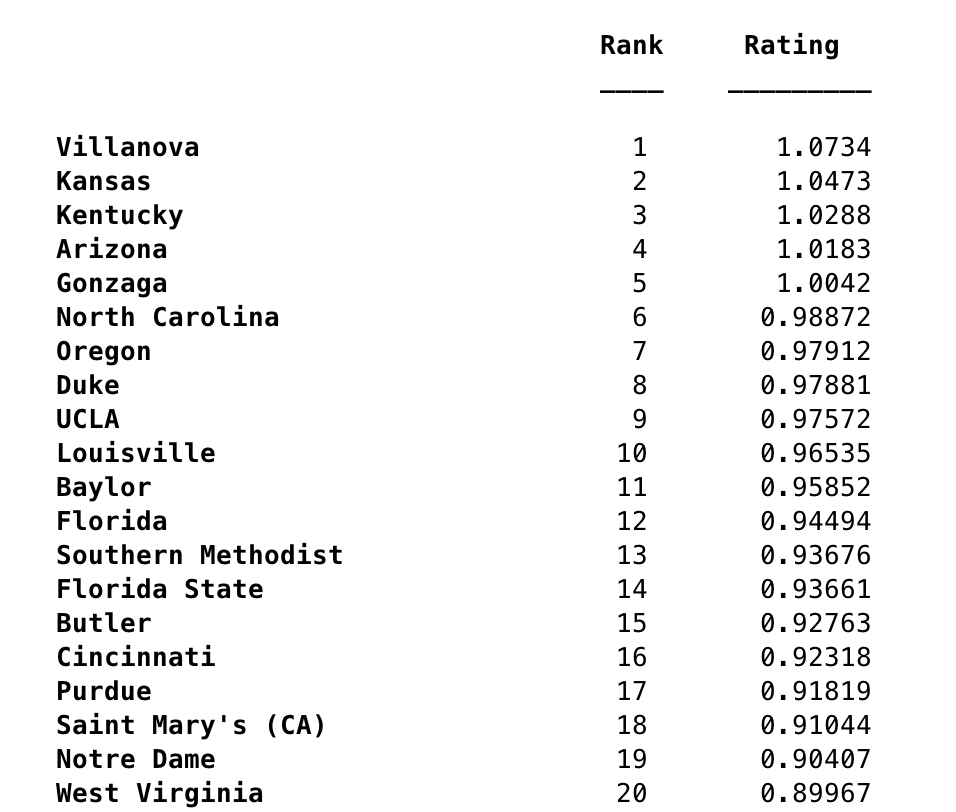
\includegraphics[width=0.8\textwidth]{Top20}
\caption{Top 20 Teams From Colley Method}
\label{fig:20Team}
\end{figure}
The average of the ranking values is 0.5 and it is quite clear to see that the top 20 teams in the nation have rankings high above the average.
\bigbreak
Since the data was organized by the date the game was played, the ELO rating for each week was easily computed in MATLAB. As with the Colley Method, the data is read in row by row (or game by game) but now the ranking of each team is instantly updated, with the performance value being determined as a 1 or 0, according to whether the team won or lost. Once every game has processed, the ranks and teams are sorted and tabulated. Just like the Colley Method, only the top 20 teams are presented below for brevity.
\begin{figure}[H]
\centering
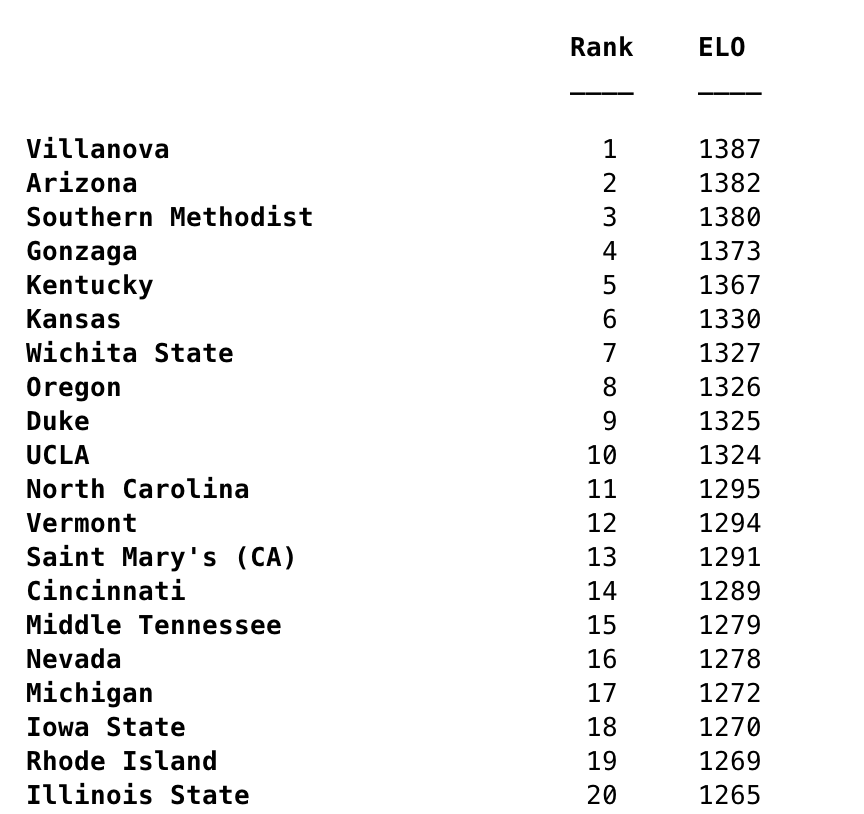
\includegraphics[width=0.8\textwidth]{Top20ELO}
\caption{Top 20 Teams From ELO Ranking}
\label{fig:20TeamELO}
\end{figure}
Comparing both ranking methods we can see that similar teams seem to stay near the same rank for the most part. There are some notable exceptions though such as Southern Methodist which is ranked 3 with ELO but 13 with the Colley Method. Furthermore, Southern Methodist was ranked 21st by the NCAA.











\section{Conclusion}
\label{sec:conc}

To start, here is a list of the top 10 teams, ranked by the NCAA Selection Committee$^{3}$, and how they compare to our Colley rank and ELO rank:
\begin{center}
\begin{tabular}{|c|c|c|c|}
\hline
Team & NCAA Rank & Colley Rank & ELO Rank \\
\hline
\hline
Villanova& 1 & 1 & 1\\ \hline
Kansas& 2 & 2 & 6\\ \hline
North Carolina & 3 & 6 & 11 \\ \hline
Gonzaga& 4 & 5 & 4\\ \hline
Kentucky& 5 & 3 & 5\\ \hline
Arizona& 6 & 4 & 2\\ \hline
Duke& 7 & 8 & 9\\ \hline
Louisville& 8 & 10 & 25\\ \hline
Oregon& 9 & 7 & 8\\ \hline
Florida State& 10 & 14 & 30\\ \hline
\end{tabular}
\end{center}
The first thing to note is that the top six NCAA Ranked teams, in a slightly different order, are the same six teams from the Colley rankings. Additionally, the ELO system ranks several teams quite differently than the Colley Method, potentially due to win/loss streaks. For the top ten NCAA teams, the average difference between the Colley rank and NCAA rank is 1.7 while the average difference between the ELO rank and NCAA rank is 5.6. Even if the outliers---Louisville and Florida State---are thrown out, the average difference between the ELO rank and NCAA rank is greater than that of the Colley rank and NCAA rank.

According to the NCAA$^{4}$, here are some selection criteria for ranking the 68 teams that make the tournament:
\begin{itemize}
\item Rating Percentage Index (RPI): win/loss for team, its opponents, and its opponents opponents'
\item Conference Results
\item Comparing common opponents
\item Box Score and key-role players
\item Strength of schedule
\item Road record
\item Historical Statistics
\item Regional Committee Input
\end{itemize}

All of these criteria are not accounted for in the Colley Method. However, if you compare the accuracy of the Colley Method with the final NCAA Ranks, they are quite similar. From testing the Colley Method on the Division-I NCAA Men's basketball teams, it is clear that using the Colley Method is a simple and computationally inexpensive way to rank teams. Although the ELO rating system is widely used and has been around for many years, the Colley method provides a simpler manner in team ranking that does not weigh results according to present strength. Instead, it averages strength over the entire season. In general, the Colley Method got closer to the NCAA ranks than the ELO system. This makes the system a great method for determining ranks at the the end of the season once all of the games have been played since it only considers the net wins and losses. Also, the Colley Method should only be hesitantly applied if team ranks are desired according to how they are doing at a particular stage of the season.

Unfortunately, any computer-based ranking system is unable to factor in everything that the NCAA Selection Committee does in order to select teams for the final tournament. However in looking at the Colley Method, it is seen that the availability of data can help closely rank teams with a computer. While most fans find magic in the chaos that is March Madness, our team found magic in the powerful information that can be found by using the Colley Method, which involves solving the simple linear system: $C$ $\vec{r}$ $=$ $\vec{b}$.










\newpage

\begin{center}
{\large\bf SUPPLEMENTARY MATERIAL}
\end{center}

\begin{description}

\item Code can be found at \texttt{github.com/bakerscott/CU-CJAM\_ColleyRankings}

\end{description}

\bigskip

\section{References}
\begin{enumerate}
\item Coll, Wesley N. Colley’s Bias Free College Football Ranking Method: (n.d.): n. pag. Princeton University. Web.
\item "Spreadsheet Sports NCAA Public." Dropbox. Spreadsheet Sports, n.d. Web. 27 Apr. 2017.
\item "March Madness Bracket: Every Seed Ranked from 68 to 1." NCAA.com. NCAA, 12 Mar. 2017. Web. 27 Apr. 2017.
\item "Men's Basketball Selections 101 - Selections." NCAA.org - The Official Site of the NCAA. N.p., 13 Feb. 2017. Web. 04 May 2017.
\item Silver, Nate. "It's Crowded At The Top Of The NCAA Tournament." FiveThirtyEight. FiveThirtyEight, 17 Mar. 2017. Web. 04 May 2017.
\item Silver, Nate. "How We Calculate NBA Elo Ratings." FiveThirtyEight. FiveThirtyEight, 09 May 2016. Web. 04 May 2017.
\end{enumerate}
\newpage




\end{document}
